\documentclass{standalone}
\usepackage{pgfplots}
\usepgfplotslibrary{fillbetween}
\pgfplotsset{compat=1.13}

\begin{document}

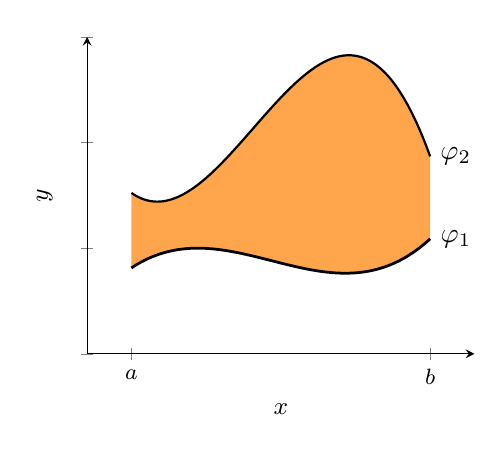
\begin{tikzpicture}
    \begin{axis}[
            axis y line = left,
            axis x line = bottom,
            xtick       = {-1.2,4.2},
            xticklabels = {$a$,$b$},
            yticklabels=\empty,
            samples     = 160,
            domain      = -1.2:4.2,
            xmin = -2, xmax = 5,
            ymin = -5, ymax = 10,
            small,
            xlabel={\(x\)},
            ylabel={\(y\)}
        ]
        \addplot[name path=top, black, thick, mark=none, ] {-x^3/3 + (x^2) + 2*x + 3} node[right]{\(\varphi_2\)};
        \addplot[name path=bottom, black, no markers, line width=1pt] {x^3/8-x^2/2} node[right]{\(\varphi_1\)};
        \addplot fill between[
                of = top and bottom,
                every even segment/.style = {orange!70},
            ];
    \end{axis}
\end{tikzpicture}

\end{document}